\newpage
\begin{center}
	\textbf{\large 4. ПРОВЕРКА СТРАТЕГИЙ НА РЫНОЧНЫХ ДАННЫХ}
\end{center}
\refstepcounter{chapter}
\addcontentsline{toc}{chapter}{4. ПРОВЕРКА СТРАТЕГИЙ НА РЫНОЧНЫХ ДАННЫХ}

В этой главе оценивается доходность стратегий инвестирования, основанных на построении оптимального портфеля Марковица,
где для прогнозирования будущих ожидаемых значений используются алгоитмы машинного обучения и модели временных рядов.
\section{Подготовка данных}

Рыночные данные были выгружены с помощью API с криптовалютной биржи OKX \cite{okx}.
В качестве доступных для торговли активов рассматриваются 8 наиболее популярных крюптовалют.
Временной период с 1 января 2022 по  1 января 2025.
Был выбран дневной таймфрейм.
Период инвестирования 1 неделя.

На графике \ref{fig:prices} изображены динамики цен активов 

\begin{figure}[H]
	\centering
	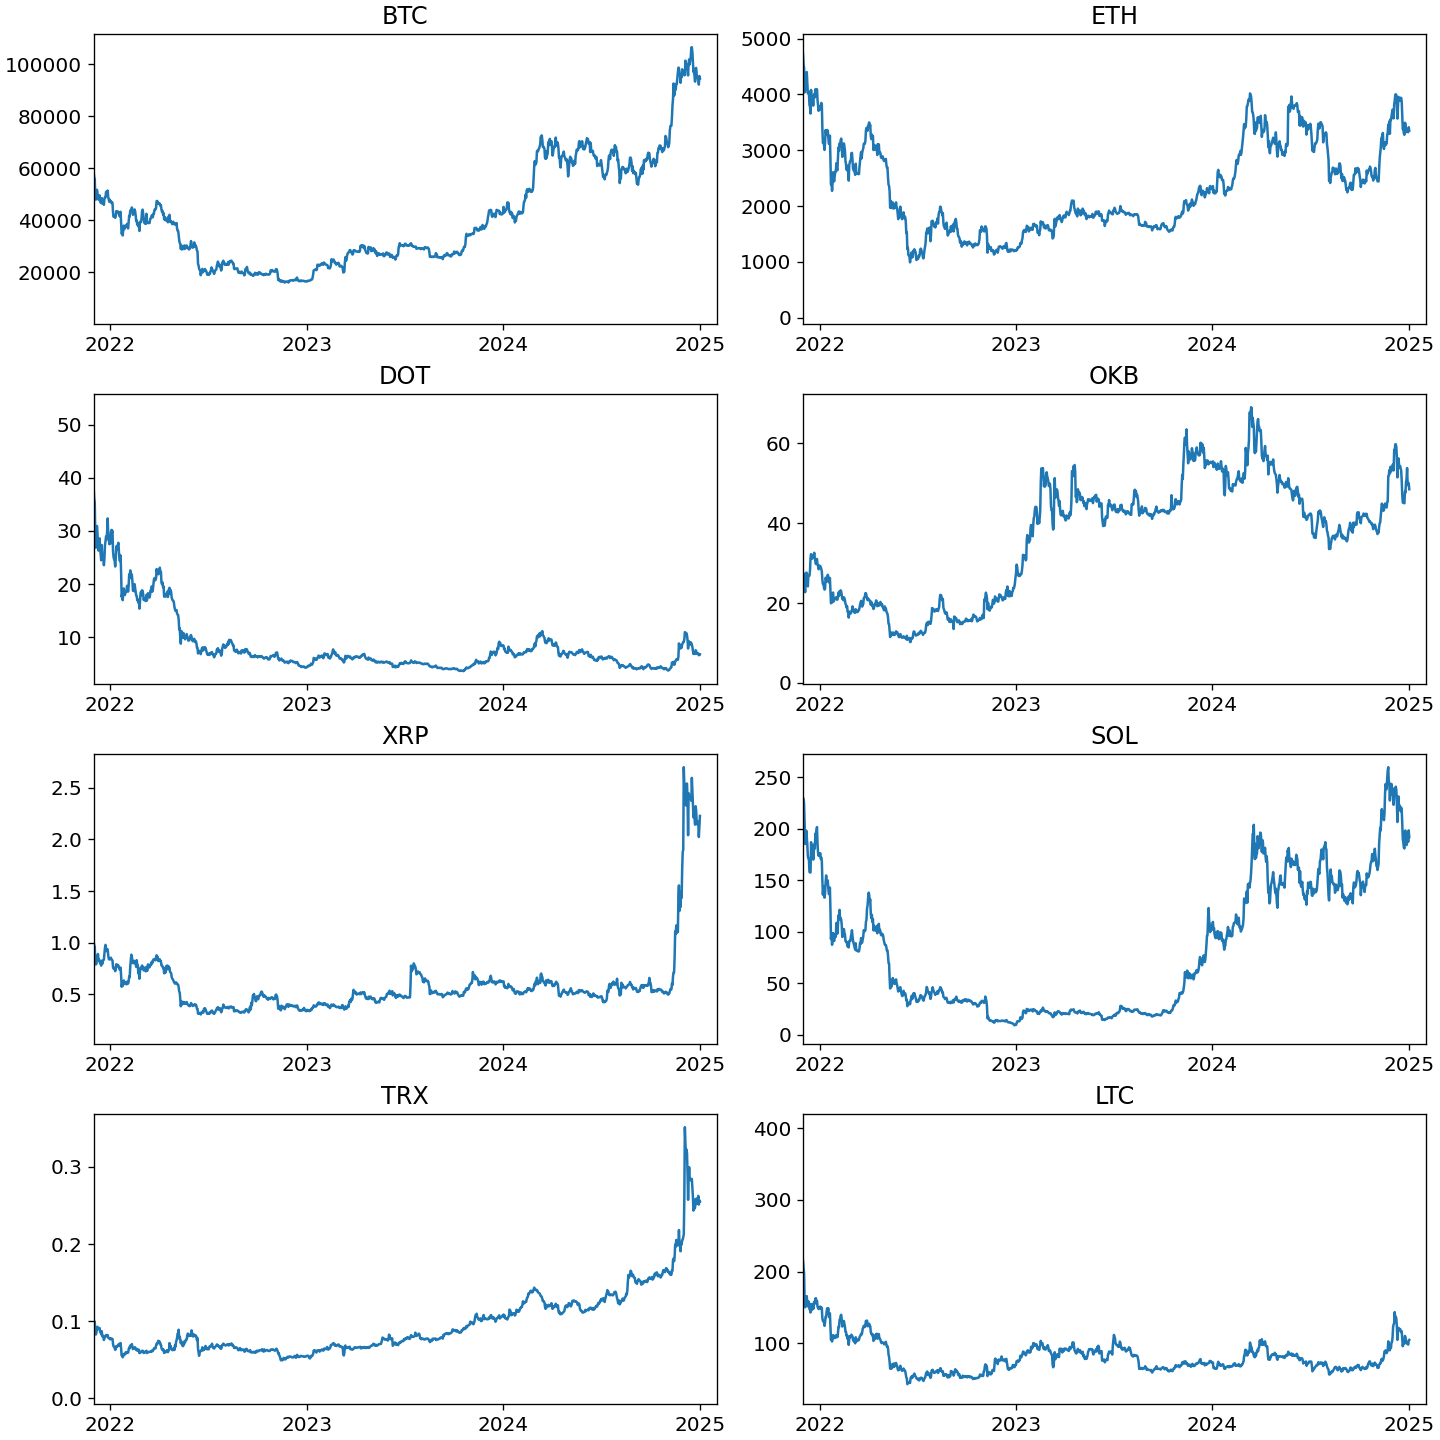
\includegraphics[width=\textwidth]{prices.png}
	\caption{Цены активов}
	\label{fig:prices}
\end{figure}

Перейдем от цен к недельным доходностям. Временные ряды соответсвующие доходностям 
представлены на графике \ref{fig:returns}, а некоторые статистики относительно распределений
доходностей в таблице \ref{tab:returns_describe}

\begin{table}[h]
\caption{Доходности активов}
\begin{tabular}{lrrrrrrrr}
\toprule
 & BTC & ETH & DOT & OKB & XRP & SOL & TRX & LTC \\
\midrule
mean & 0.0073 & 0.0038 & -0.0031 & 0.0077 & 0.0132 & 0.0114 & 0.0105 & 0.0025 \\
std & 0.0779 & 0.0961 & 0.1110 & 0.0936 & 0.1328 & 0.1482 & 0.0800 & 0.1001 \\
min & -0.3328 & -0.3830 & -0.3925 & -0.3591 & -0.3596 & -0.6018 & -0.3162 & -0.3392 \\
25\% & -0.0358 & -0.0477 & -0.0724 & -0.0401 & -0.0506 & -0.0765 & -0.0236 & -0.0513 \\
50\% & 0.0026 & -0.0013 & -0.0084 & -0.0016 & -0.0003 & -0.0034 & 0.0106 & 0.0001 \\
75\% & 0.0446 & 0.0555 & 0.0573 & 0.0494 & 0.0430 & 0.0906 & 0.0373 & 0.0546 \\
max & 0.3566 & 0.5056 & 0.6188 & 0.4003 & 1.0235 & 0.7409 & 0.7407 & 0.5294 \\
\bottomrule
\end{tabular}
\label{tab:returns_describe}
\end{table}


\begin{figure}[H]
	\centering
	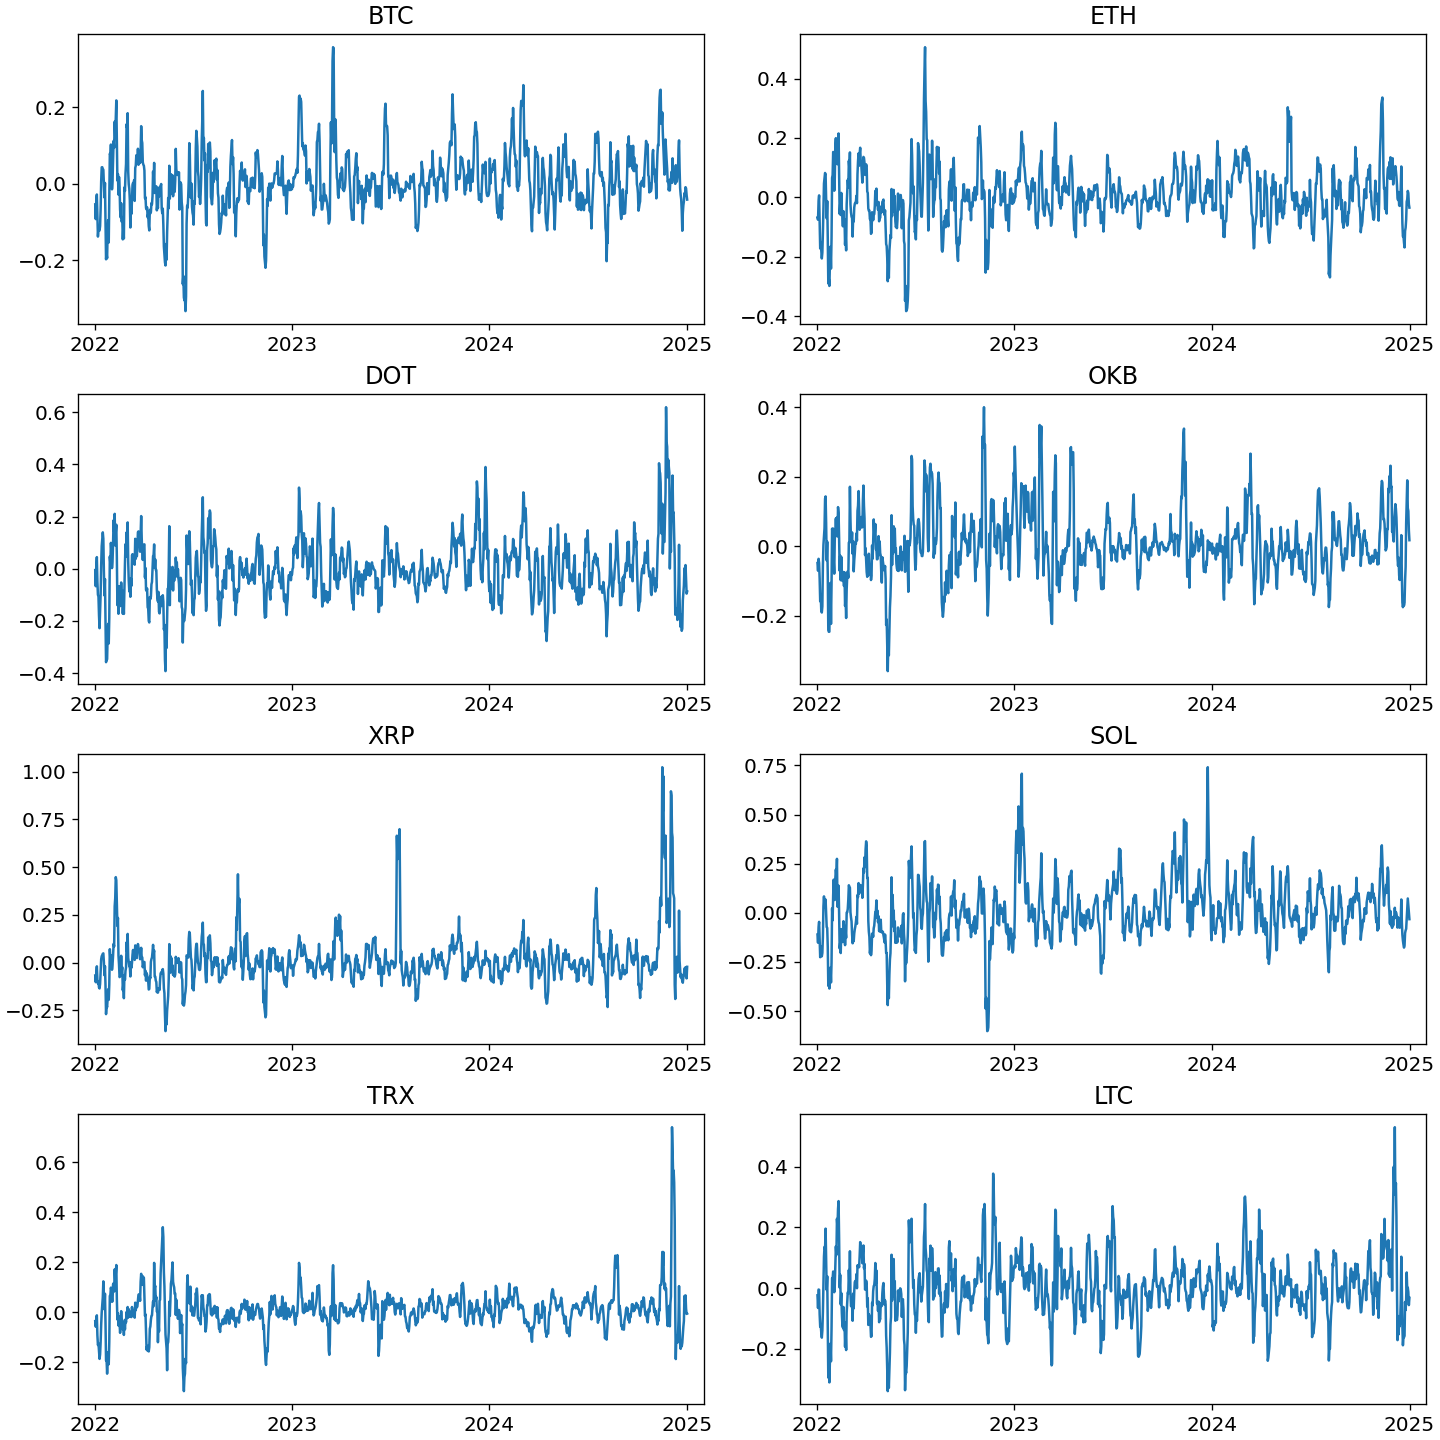
\includegraphics[width=\textwidth]{returns.png}
	\caption{Доходности активов}
	\label{fig:returns}
\end{figure}
Можно видеть редкие но достаточно сильные скачки.

Распределение доходностей активов представлено на гистограммах на рисунке \ref{fig:rois_hist}

\begin{figure}[H]
	\centering
	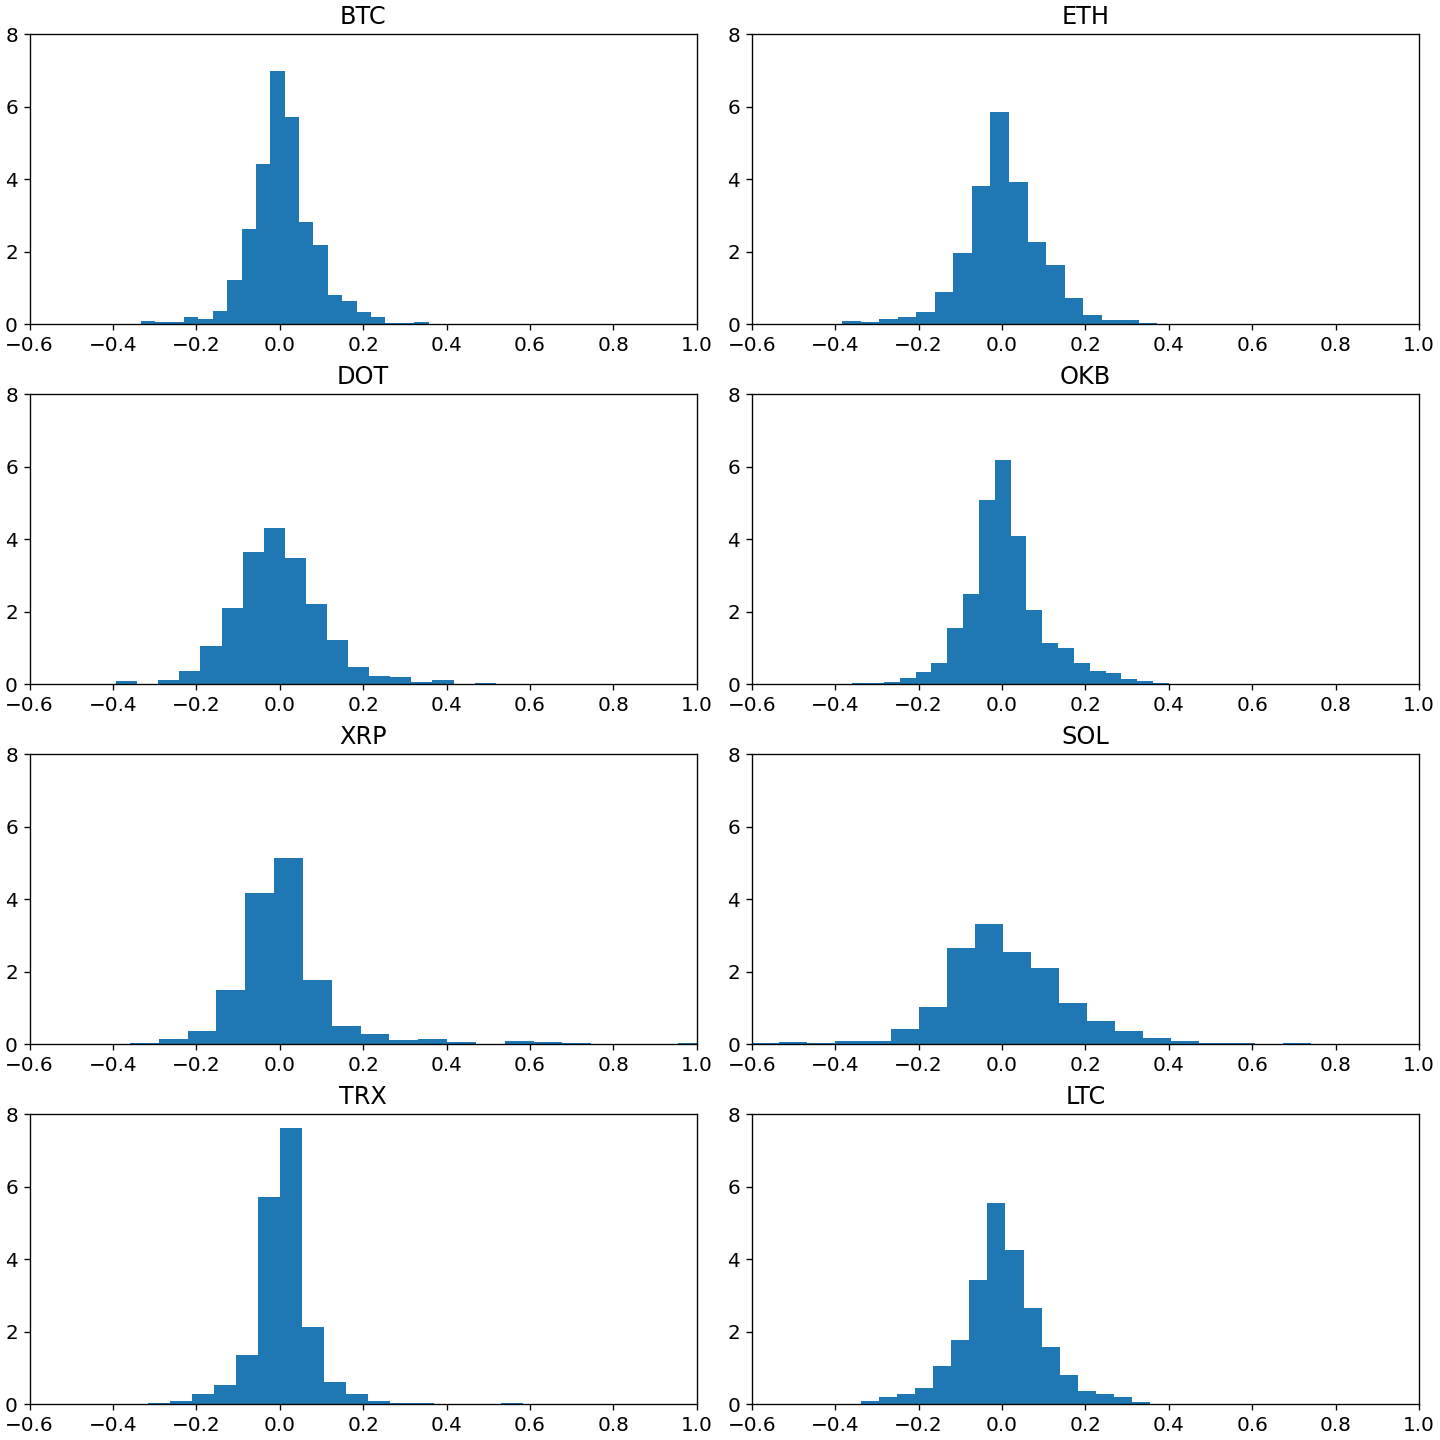
\includegraphics[width=\textwidth]{rois_hist.png}
	\caption{Гистограммы доходностей активов}
	\label{fig:rois_hist}
\end{figure}

Из гистограмм видно, что распределение доходностей унимодально и имеет тяжелый правый хвост.

На графике \ref{fig:rois_mean_std} сравниваются активы с точки зрения 
среднего и стандартного отклонения доходности.

\begin{figure}[H]
	\centering
	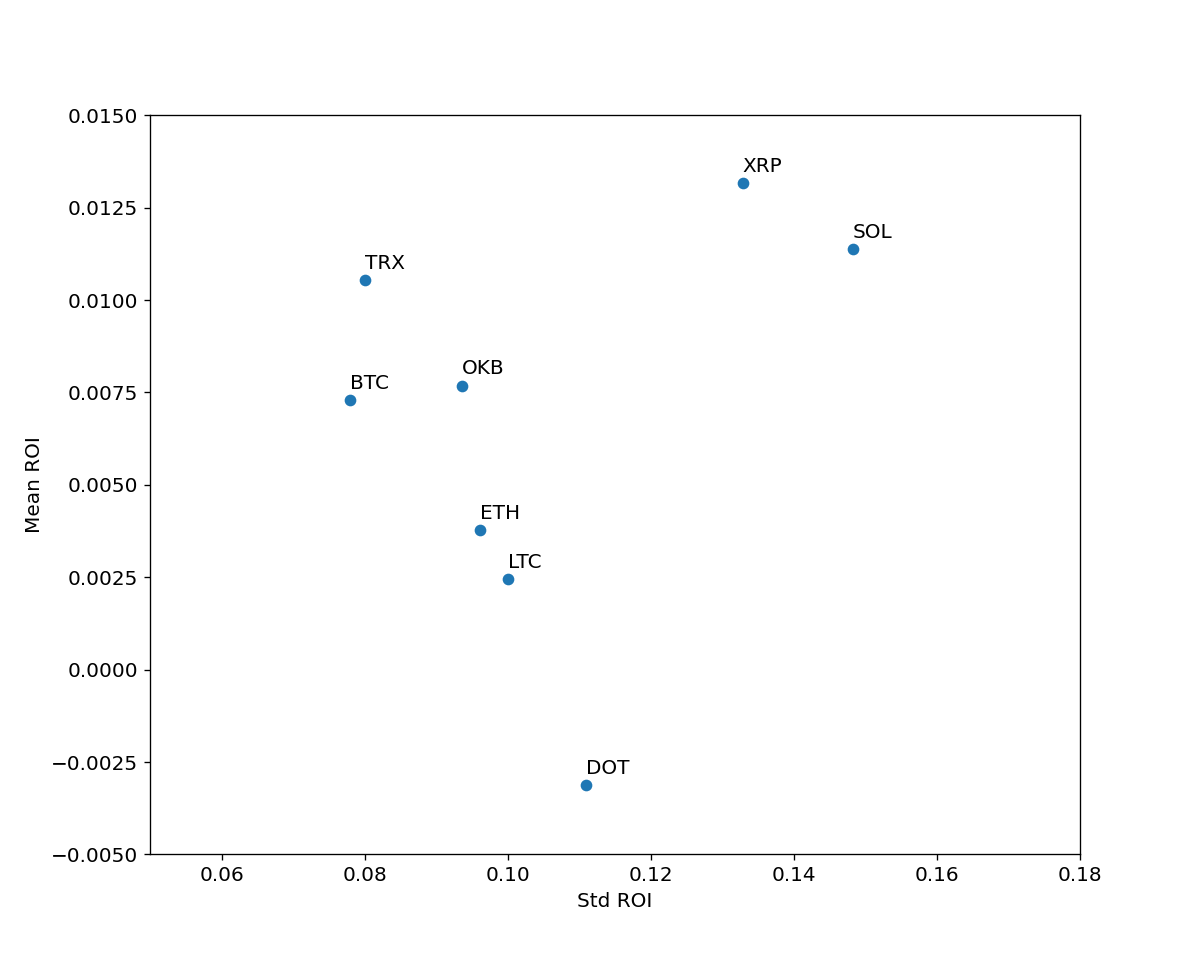
\includegraphics[width=\textwidth]{rois_mean_std.png}
	\caption{Среднее и стандартное отклонение доходностей}
	\label{fig:rois_mean_std}
\end{figure}

Разделим имеющиеся данные на валидационную и тестовую выборки. В качестве тестовых данных возьмем 2024 год.
По валидационной выборке подберем гиперпараметры для модели из каждого рассматриваемого класса.

В дальнейшем тестовые данные будут использоваться для:
\begin{enumerate}
	\item оценки качества прогнозирования средней ожидаемой доходности
	\item тестирования портфельных стратегий
\end{enumerate}

Из тестовых днных формируется набор тест-кейсов на которых и оценивается качество.
Процесс формирования тест-кейсов схематично проилюстрирован на рисунке \ref{fig:ts_csv}.
\begin{figure}[H]
	\centering
	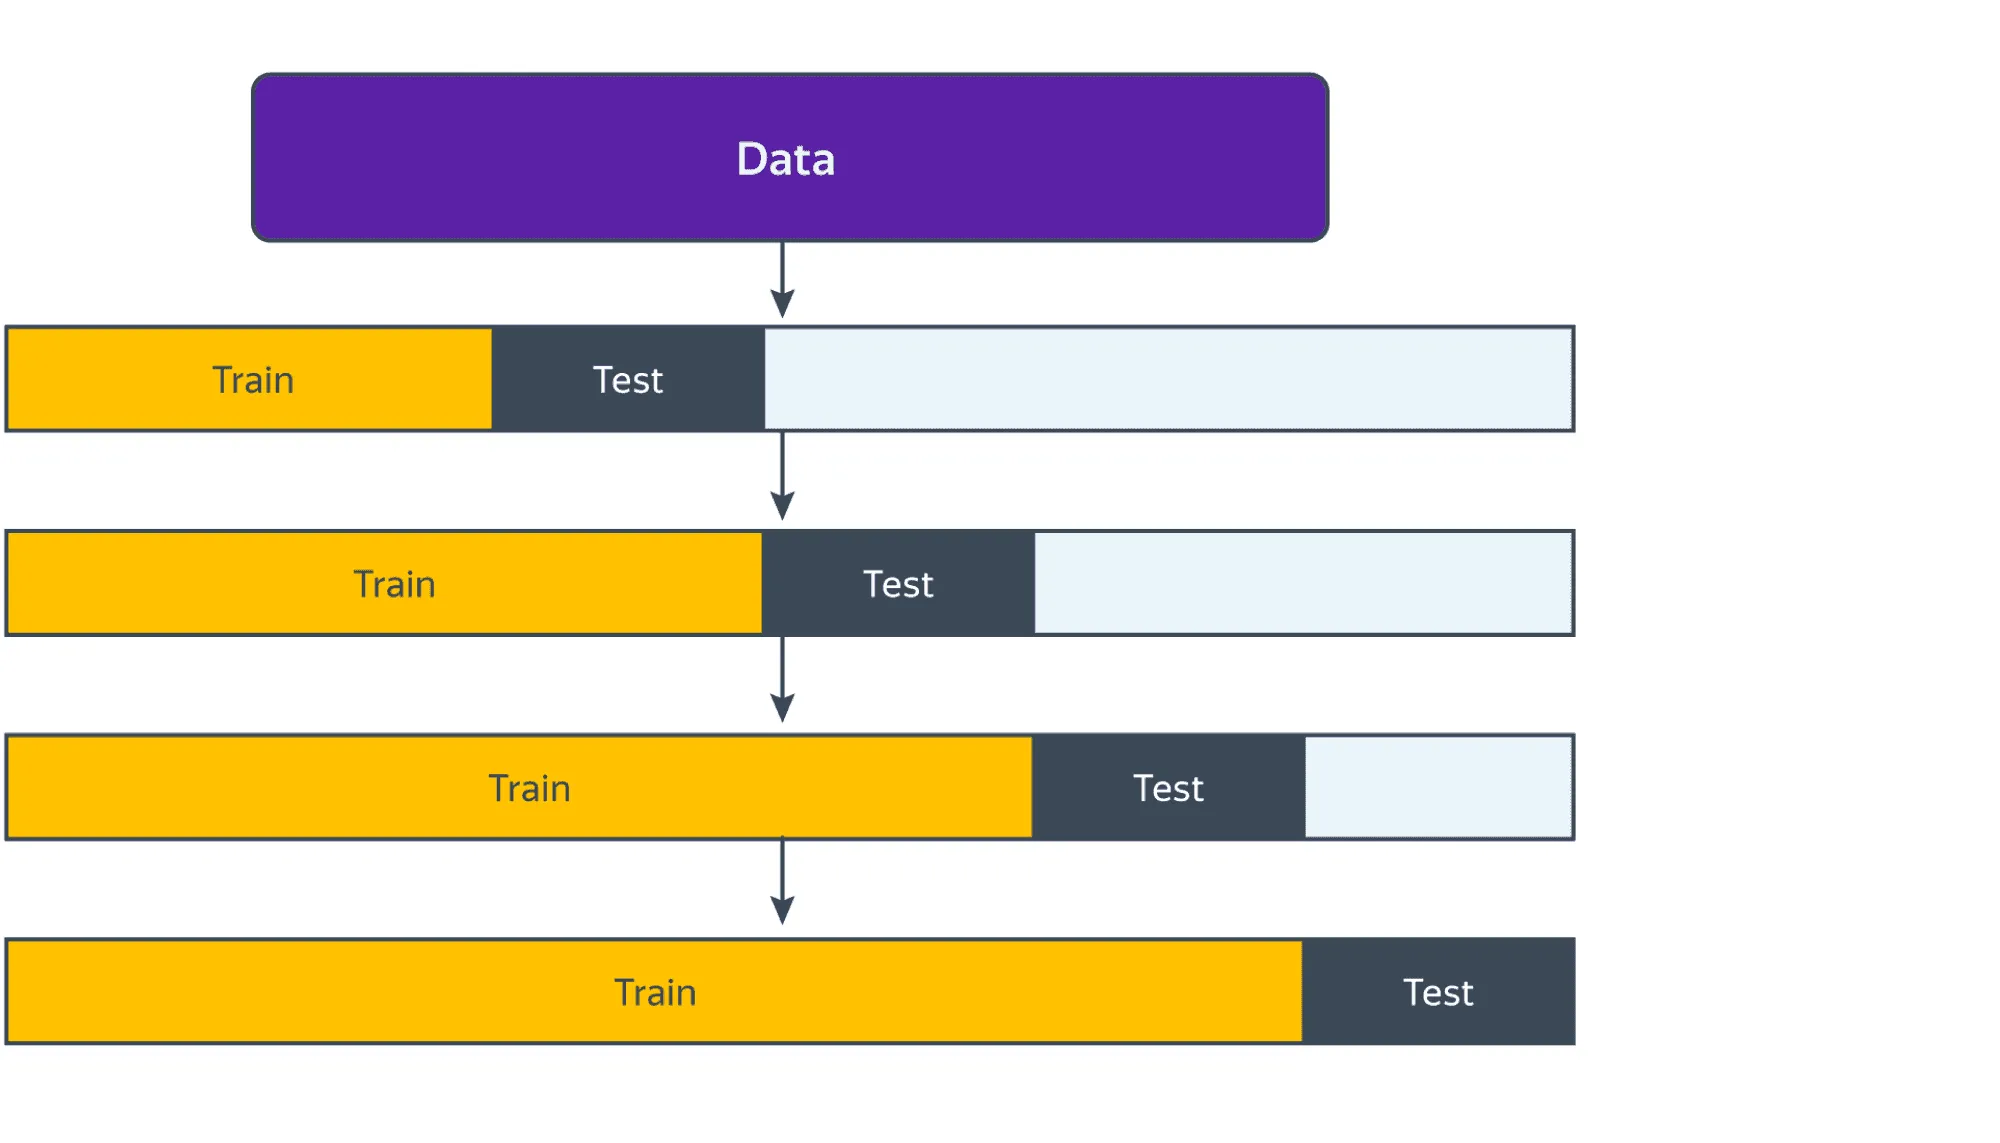
\includegraphics[width=\textwidth]{images/ts_cv}
	\caption{Формирование тест-кейсов из тестовых данных}
	\label{fig:ts_csv}
\end{figure}

Следующим этапом идет расчет необходимых параметров для оптимизации портфеля --- 
оценка ковариаций и прогноз средних значений доходности.

\section{Оценка ковариации между активами}

Особую сложность предстваляет задача прогноза будущей ковариации временных рядов. 
Вполне естественным вляется предположение стационарности ковариации во времени. 
Поэтому воспользуемся выборочной оценкой ковариации по историческим данным.

Имея $r_t$ - вектор-столбец доходностей в момент времени t, по истории наблюдений $r_1, \cdots r_n$ 
выборочная ковариация $\Sigma$ рассчитывается как 
\begin{align}
	\Sigma = \frac{1}{n} \sum_{t=1}^{n}(r_t - \overline{r}) \cdot (r_t - \overline{r})^T
\end{align}
где $\overline{r} = \frac{1}{n} \sum_{t=1}^{n} r_t$.

Корреляция Пирсона между доступными активами представлена на рисунке \ref{fig:corr}.

\begin{figure}[H]
	\centering
	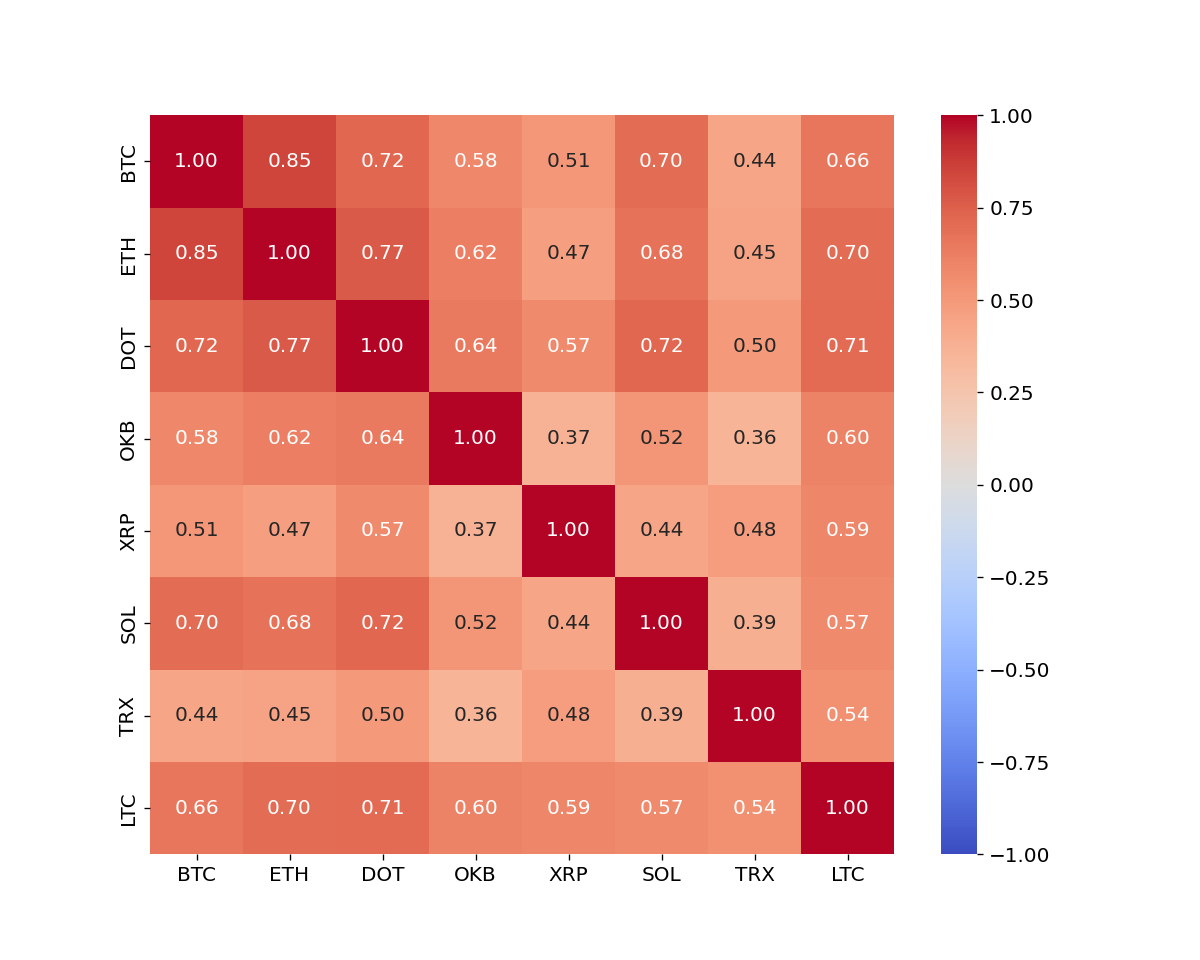
\includegraphics[width=\textwidth]{corr.png}
	\caption{Корреляции доходностей активов}
	\label{fig:corr}
\end{figure}

Активы имею сильную положительную корреляцию.

\section{Модели оценки средней доходности}

Задача оценки средней ожидаемой доходности сводиться к умению прогнозировать значение основываясь на стории наблюдений.
Для этого подходят классические статистические модели, модел имашинного обучения и нейросети в адаптации для прогнозирования 
временных рядов.

Ограничемся рассмотрением следующих моеделей:
\begin{enumerate}
	\item NAIVE - выборочное среднее
	\item MARTINGAL - прогноз последним наблюдаемым значением 
	\item ARIMA - модель авторегрессии и скользящего среднего
	\item LR - линейная регрессия
	\item RF - случайный лес
\end{enumerate}

Для каждого актива будем строить отдельную модель не принимающую в расчет историю других активов.
Таким образом, для прогноза будующих доходностей активов необходимо построить моделей по числу активов.

Некоторые модели (ARIMA, RF) --- допускают свободу в выборе гиперпараметров. 
Подбор гиперпараметров моделей осуществлялся по тренировочной выборке.

Качество прогнозирования моделей оценивается с помощью среднеквадратичной ошибки MSE (Mean Squared Error):
\begin{align}
	MSE = \frac{1}{n} \sum_{i=1}^{n} (r_i - \hat{r}_i)^2
\end{align}
где $r_i$ - истинное значение доходности,
а $\hat{r}_i$ - прогнозное значение модели на $i$-м объекте тестовой выборки.

Результаты оценки качества прогнозирования на тестовых данных представлены в таблице \ref{tab:ml_eval_metrics}

\begin{table}[h]
\caption{Качество прогнозирования MSE$\cdot 10^4$}
\label{tab:ml_eval_metrics}
\begin{tabular}{lrrrrr}
\toprule
 & NAIVE & MARTINGAL & LR & ARIMA & RF \\
\midrule
BTC & 5.63 & 1.20 & 1.58 & 1.62 & 2.07 \\
ETH & 8.00 & 1.99 & 4.47 & 3.70 & 5.05 \\
DOT & 16.51 & 3.89 & 4.09 & 3.98 & 5.28 \\
OKB & 6.06 & 1.56 & 1.77 & 1.95 & 2.05 \\
XRP & 24.33 & 5.04 & 6.98 & 5.71 & 6.53 \\
SOL & 21.19 & 4.47 & 11.86 & 6.16 & 5.31 \\
TRX & 7.96 & 1.85 & 4.19 & 5.30 & 6.04 \\
LTC & 8.53 & 2.66 & 2.24 & 3.22 & 5.11 \\
\bottomrule
\end{tabular}
\end{table}


Наихудшее значениие показывает подход NAIVE.
Это обусловлено резким ростом цен в 2024 году после относительно спокойной динамики.
MARTINGAL показывает хорошие результаты в случае рядов с затяжным трендов.
Остальные модели показывают сопоставимое качество.

\section{Проверка стратегий на тестовых данных}

Под стратегией будем понимать некоторый принцип или алгоритм по которому в каждый момент времени
формируется портфель.
Будем рассматривать стратегии двух видов:
\begin{itemize}
	\item тривиальные 
	\item основанные на идеи Марковица
\end{itemize}

Среди тривиальных стратегий выберем следующие:
\begin{enumerate}
	\item UNIFORM - равномерное инвестированиие во все доступные активы
	\item MOST RISKY - актив с наибольней дисперсией доходности
	\item LESS RISKY - актив с наименьшей дисперсией доходности
	\item BEST RETURN - актив с наибольшей средней доходностью
	\item WORST RETURN - актив с наименьшей средней доходностью
\end{enumerate}

Стратегии Марковица определяются риск-параметром и моделью оценки средней ожидаемой доходностью.
Риск-параметр будем воспринимать как параметризацию класса стратегий с определенной моделью оценки средней ожидаемой доходности.
Таким образом, одной стратегии Марковица соответсвует множество стратегий с разным риск-параметром. 
Это множество стратегий будет называть фронтирой.

На каждом тест-кейсе с помощью стратегии формируется инвестиционный портфель
в расчете на единичную сумму инвестирования и оценивается доходность ROI (Return On Investment) полученного портфеля.

На графике \ref{fig:result_frontier} представлены фронтиры соответсвующие торговым стратегиям.
Серым цветом отмечены тривиальные портфели.
По оси абсцисс отложены стандартые отклонения ROI, а по оси ординат --- средние значение ROI.

\begin{figure}[H]
	\centering
	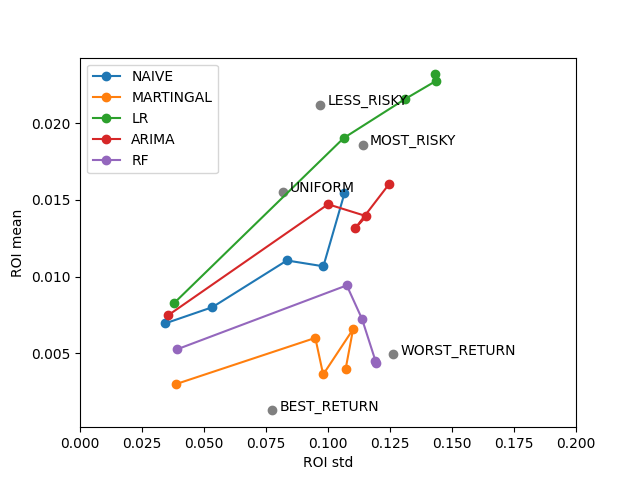
\includegraphics[width=\textwidth]{result_frontiers.png}
	\caption{Результаты тестирования стратегий}
	\label{fig:result_frontier}
\end{figure}

Более детально средние значения и стандартные отклонения ROI стратегий представлены в таблицах
\ref{tab:roi_mean} и \ref{tab:roi_std} соответственно.

Метрики тривиальных портфелей представлены в таблице \ref{tab:trivial_rois}

\begin{table}[h]
\caption{Средние ROI $\cdot 10^3$}
\label{tab:roi_mean}
\begin{tabular}{lrrrrr}
\toprule
 &  0.01 &  0.26 &  0.51 &  0.75 &  1.00 \\
\midrule
NAIVE & 6.9451 & 8.0025 & 11.0462 & 10.6657 & 15.4227 \\
MARTINGAL & 2.9859 & 6.0019 & 3.6178 & 6.5656 & 3.9942 \\
LR & 8.2600 & 19.0185 & 21.5537 & 22.7442 & 23.1668 \\
ARIMA & 7.4648 & 14.7066 & 13.9296 & 13.1520 & 15.9971 \\
RF & 5.2633 & 9.4236 & 7.2398 & 4.3777 & 4.5050 \\
\bottomrule
\end{tabular}
\end{table}


\begin{table}[h]
\caption{Стандартное отклонение ROI $\cdot 10^2$}
\label{tab:roi_std}
\begin{tabular}{lrrrrr}
\toprule
 &  0.01 &  0.26 &  0.51 &  0.75 &  1.00 \\
\midrule
NAIVE & 3.4328 & 5.3375 & 8.3427 & 9.8131 & 10.6650 \\
MARTINGAL & 3.8577 & 9.4886 & 9.8051 & 11.0111 & 10.7128 \\
LR & 3.7892 & 10.6314 & 13.1000 & 14.3570 & 14.3071 \\
ARIMA & 3.5454 & 10.0037 & 11.5506 & 11.1001 & 12.4518 \\
RF & 3.9215 & 10.7564 & 11.3710 & 11.9397 & 11.9118 \\
\bottomrule
\end{tabular}
\end{table}


\begin{table}[h]
\caption{Тривиальные портфели}
\label{tab:trivial_rois}
\begin{tabular}{lrr}
\toprule
 & mean ROI $\cdot 10^3$ & std ROI $\cdot 10^2$ \\
\midrule
UNIFORM & 15.5372 & 8.1775 \\
MOST RISKY & 18.5904 & 11.3970 \\
LESS RISKY & 21.1635 & 9.6881 \\
BEST RETURN & 1.2790 & 7.7329 \\
WORST RETURN & 4.9217 & 12.6324 \\
\bottomrule
\end{tabular}
\end{table}


